%%% -*-LaTeX-*-

\chapter{Introduction}

\setupuuchapterbib
%
In many domains of science and engineering, a software developer needs to implement a real-valued mathematical formula or algorithm on a computer.
%
Unfortunately, the developer cannot simply transcribe the formula or algorithm \textquotesingle\textquotesingle from the paper\textquotesingle\textquotesingle \space into the computer using their programming language of choice.
%
The main reason is that computers calculate with finite resources, while in our ideal formula or algorithm, we compute in real arithmetic, and thus with a potentially infinite number of digits.
%
In mathematics there are quantities, for example $\pi$ or $\sqrt{2}$ or any other irrational number, with an infinite number of digits, which cannot be represented \emph{exactly} using a finite machine representation.
%
%Similar argument holds for rational numbers with many digits. 
%
Such numbers have to be \emph{rounded} to fit the finite representation, and the gap between the real number and the rounded counterpart is called \emph{roundoff error}.
%

%
Computers store numbers in the form of a finite sequence of binary digits, which \emph{unavoidably} result in inaccurate real-valued computations.
%
The precision format (often called \emph{bit-width} in the literature) is the length of the sequence used to represent numbers in computers.
%
As a rule of thumb, the wider the precision format the more accurate the computations are.
%
Hence, a naive software developer might want to use a high bit-width format, like for example 10000 bits, to mimic real arithmetic as best as possible. 
%
However, this is typically not a viable option in practice.
%

First, computing using a finite precision format results in roundoff errors regardless of the bit-width being used.
%
To put it simply, computing with 10000 bits is not the same as computing with infinite bits.
%
Indeed, finite-precision arithmetic does not respect the rules of real arithmetic done with \textquotesingle \textquotesingle pen and paper\textquotesingle\textquotesingle.
%
For example, the associativity law from real arithmetic fails in finite-precision where it is often the case that $(a*b)*c \ne a*(b*c)$.

Second, high bit-width formats are very expensive in terms of compute resources which include, among others, energy-consumption, execution time, and the physical space of the floating-point unit on the board~\cite{fppower, lutnet}. 
%
The usage of resources is critical on portable devices, like smart-phones or smart-watches, where the battery consumption is a primary concern, as well as supercomputers, which consume large amounts of electrical power.
%
Moreover, when dealing with chips with size in the order of square millimeters, like micro-controllers, or where the available memory is very limited, in the order of a kilobyte, it is impossible to compute using high bit-width formats.

%
We have to live with the fact the arithmetic in computers is imprecise.
%
On the other hand, we cannot simply ignore the roundoff error stemming from the use of finite-precision arithmetic, because it can have catastrophic consequences on the correct execution of the program.
%

For example, consider the C program reported in Figure~\ref{fig:while}.
%
\begin{figure}[b!]
	\begin{lstlisting}[frame=single, language=c]
  float    f = 0;
  double   d = 0;
  int      n = 0;
  int      limit=0;
  scanf("%d", &limit);
  for (int i = 0; i < limit; i++){
    f = f + 0.1;
    d = d + 0.1;
    n = n + 1.0;
  }
  printf("%.50f\n", f);
  printf("%.50f\n", d);
  printf("%d\n", n);
	\end{lstlisting}
	\caption{A simple C program with an imprecise accumulator showing the effect of roundoff errors.}\label{fig:while}
\end{figure}
%
The program instantiates one single-precision floating-point variable \emph{f}, one double-precision floating-point variable \emph{d}, and an integer variable \emph{n}.
%
In the body of the for-loop, we increment the float \emph{f} and the double \emph{d} by the constant value 0.1, while we increment the integer variable \emph{n} by one.
%
The number of iterations of the for-loop is user-defined through the variable \emph{limit}.
%
When we run our program with the \emph{limit} set to $10^6$, the value of the variable \emph{f} after the for loop is roughly 100958.34, while the value of \emph{d} is roughly 100000.0000013. The value of \emph{n} matches exactly $10^6$.
%
Ideally, both \emph{f} and \emph{d} should be $10^5$, thus there is an absolute error of 958.34 in float and 0.0000013 in double.
%
We run our program a second time with \emph{limit} set to $10^8$. 
%
After the loop, the value of \emph{f} and \emph{d} are respectively 2097152.0 and 9999999.98, thus there are absolute errors of 7902848.0 and 0.02. 
%
Again, the value of \emph{n} matches the limit exactly.
%
The reason behind such roundoff errors is that the decimal constant 0.1 is not exactly representable in binary (see Section~\ref{fpsection} for a detailed explanation). 

%
From an implementation perspective, a similar issue was the cause of the Patriot Missile Failure~\cite{patriot}.
%
In 1991, during the Gulf War, an American Patriot Missile Defense battery failed to intercept an incoming missile.
%
The cause of the failure was the internal clock, in the Patriot battery, used to measure time in tenths of second.
%
This number was then multiplied by the decimal constant 0.1, which we know is not exactly representable, to produce the time in seconds.
%
The Patriot battery had been up and running for about 100 hours, and follow-up investigations showed the accumulated roundoff error corresponded to a travel time of 0.34 seconds for an incoming missile. 
%
In this amount of time, the incoming missile could travel for about half a mile.
%

Roundoff errors are everywhere, and they can have catastrophic consequences on the correct execution of a program.
%
Therefore, this dissertation aims to address the problem of the analysis of roundoff errors in floating-point computations.
%
\section{Computation Errors}
%

Finite-precision arithmetics, like floating-point, make mathematics feasible on computers. 
%
Regardless of the base used for the representation (base 2 nowadays), not all real numbers can be exactly represented using a finite number of bits.
%
For example, periodic and irrational numbers, like $\frac{1}{3}$ and $\pi$, have to be rounded to fit the format of the representation. 
%
%The wider the format used for the representation, the smaller the gap between the real value and the value stored in the machine.
%
%In this thesis, we represent computed quantities with a hat (e.g., $\widehat{x}$) to distinguish from the real counter-part (e.g., $x$).
%
The most common ways to express roundoff errors in computers are the absolute error and the relative error~\cite{higham2002accuracy}.
%

Let $\widehat{x}$ be the finite precision representation of $x$. Then, we define the absolute error as
%
\begin{align}
Err_{abs}=|x-\widehat{x}|\label{absolute}
\end{align}
%
while the relative error is
%
\begin{align}
Err_{rel}=\frac{|x-\widehat{x}|}{x}\label{relative}
\end{align}
%
The magnitude of the absolute error depends on the magnitude of the computations.
%
In floating-point arithmetic, where numbers are equally spaced only within the same exponent range (between perfect powers of two), the relative error is more of interest because it is scale independent.
%
In other words, as opposed to the absolute error, the magnitude of the relative error is independent from the magnitude of the computation itself.
%

%On the other hand, anytime the real computation involves the value zero the relative error is undefined.
%
When the denominator in Equation (\ref{relative}) is zero, the fraction is undefined and thus the concept of the relative error is not applicable.
%
Investigating the roundoff error in a neighborhood of zero is of special importance in numerical analysis, mainly because of underflow or cancellation phenomena~\cite{every}. Thus, in many practical applications we do want to study the roundoff error when the real computation does involve the value zero, which leaves us with only the absolute error measure.
%
\section{Floating-Point Arithmetic}
\label{fpsection}
%
\begin{table}[b]
	\centering
	\newcommand{\mydashline}{\hdashline[1pt/1pt]}
	\scriptsize
	\renewcommand{\arraystretch}{1.5}
	%\setlength{\tabcolsep}{0.3em} % for the horizontal padding
	%		Benchmark & \Tool & Sampling & Golden & PrAn& \Tool & Sampling & Golden & FpTaylor\\
	\begin{tabular}{@{\extracolsep{2.3pt}}p{1.5cm}L{1.2cm}L{1.2cm}L{1.3cm}@{}}
		\toprule
		%\multirow{4}{*}{Benchmark} & \multicolumn{2}{c}{uniform} & \multicolumn{2}{c}{normal} & \multicolumn{1}{c}{exp} &\multirow{4}{1.2cm}{FpTaylor}\\
		%\cmidrule{2-3} \cmidrule{4-5} \cmidrule{6-6}
		\multicolumn{1}{c}{Format (bits)}& \multicolumn{1}{c}{Mantissa} & \multicolumn{1}{c}{Exp} & \multicolumn{1}{c}{$\epsilon$}\\
		\midrule
		half (16) & 10 & 5 & 4.88e-4 \\
		\mydashline{}
		single (32) & 23 & 8 & 5.96e-8 \\
		\mydashline{}
		double (64) & 52 & 11 & 1.11e-16 \\
		\mydashline{}
		quad (128) & 112 & 15 & 9.63e-35 \\
		\bottomrule
	\end{tabular}
	\caption{IEEE-754 floating-point formats. We report the name of the format (Format) and the bit-width for the mantissa (Mantissa) and the exponent (Exp) representations. The column $\epsilon$ reports the value of machine epsilon.}
	\label{fpformat}
\end{table}
%
The floating-point system, as specified in the IEEE 754 standard~\cite{ieee754}, is a subset of the reals.
%
A floating-point number consists of the triple \emph{sign}, \emph{mantissa}, and \emph{exponent}.
%
We compute the value of the triple as $\;\text{-}1^{sign}*mantissa*2^{exponent}$.
The sign is always one bit, with value 0 for positive or 1 for negative numbers, while the bit-width of the mantissa and the exponent are format-dependent.
%

%
Table~\ref{fpformat} reports the formats of the most common binary data-types in the standard.
%
The standard defines, among others, the widely used single and double data-types, with 32 and 64 bits formats, and several rounding modes.
%
Rounding is used when the exact result of a computation does not fit the finite precision format.
%
The default rounding mode in the standard, round-to-nearest, rounds the ideal result of the computation to the nearest representable floating-point value.
%
In case of a tie, the floating-point value ending with zero is chosen.
%
From the point of view of numerical analysis it is important to understand that floating-point numbers are not evenly distributed in the real line~\cite{every}.
%
%There are the same number of floating-point numbers within two consecutive powers of two (see Figure~\ref{fig:line}).
%
Indeed, they are evenly spaced only within two consecutive powers of two, as Figure~\ref{fig:line} illustrates.

%
\begin{figure}[b!]
	\centering
	\begin{tabular}{l}
		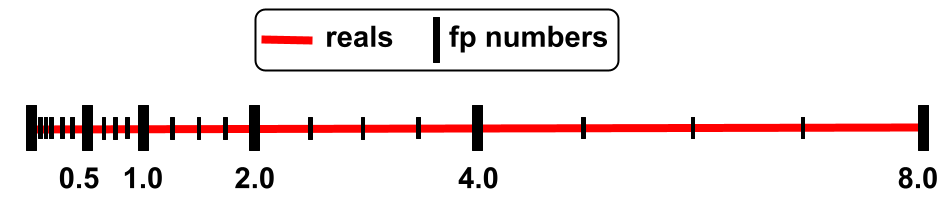
\includegraphics[width=1.0\textwidth]{pic/fpnumbers.png}
	\end{tabular}
	\caption{The spacing between floating-point numbers (black-and-white squares), plotted on the top of the real line (red), is uniform only within two consecutive powers of two.}
	\label{fig:line}
\end{figure}
%
\begin{figure}[b!]
	\centering
	\begin{tabular}{l}
		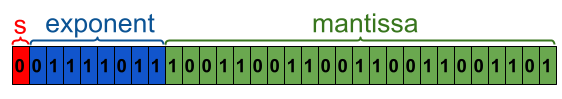
\includegraphics[width=1.0\textwidth]{pic/examplenumber.png}
	\end{tabular}
	\caption{Single precision floating-point representation of the decimal value 0.1 using the default rounding mode round-to-nearest.}
	\label{fig:zeropointone}
\end{figure}
%

Assuming the computation does not overflow or underflow, the standard model of floating-point arithmetic~\cite{every} states
%
\begin{align}
rnd(x)=x(1+e),\;\;\;\text{where}\;\;\;|e|\leq\epsilon
\label{standard}
\end{align}
%
where $rnd(x)$ is the floating-point value of the real computation $x$, and the error $e$ is bounded by the so-called \emph{machine epsilon}, that is the upper-bound on the relative error.
%
Table~\ref{fpformat} reports the value of $\epsilon$ for each format in the standard.
%
For example, for single-precision $\epsilon=2^{-24}$, while for double-precision $\epsilon=2^{-53}$.
%
The standard model in Equation~(\ref{standard}) holds for normal numbers, which are the focus of this dissertation.
%
Note that the model would be slightly more complex if we were to also consider subnormal numbers, but these are ignored here since we do not support subnormals in the contributions of this dissertation.
%

In Figure~\ref{fig:zeropointone}, we report the format representation when the decimal real value 0.1 is stored in a single precision (32 bits) floating-point variable.
%
The decimal value $0.1$ becomes $0.0\overline{0011}$ in binary, which in normalized form is $1.1\overline{0011}*2^{\text{-}4}$.
%
This number is periodic, hence it is not exactly representable in single --- or any other finite --- precision format.
%

Let us discuss the details of the format representation.
%
The sign is zero because the number is positive.
%
The stored value for the exponent corresponds to the decimal 123, on the other hand, we saw the actual value of the exponent should be -4.
%
This is because the stored exponent is shifted, with respect to the actual value, by the exponent bias. 
%
Thanks to the bias, the exponent is stored as unsigned number, as opposed to signed number, which makes an eventual comparison with other floating-point numbers in the future easier.
%
The bias is computed as $2^{exp\text{-}1}\text{-}1$, where $exp$ is the number of bits for the exponent representation, and then, it is added to the actual value of the exponent.
%
Thus, if we go back to our example, we have $\text{- }4\text{ + }2^{(8\text{-}1)}\text{ - }1=123$.
%
Finally, the last part of the format is for the mantissa representation. 
%
For normal numbers, like 0.1 in our example, the IEEE standard assumes there is always an implicit leading bit, set to one, which is not actually stored in the representation.
%
%In other words, the actual value of the mantissa is obtained by placing a leading 1$1.$\emph{mantissa}.
%
This is called the hidden or implicit bit.
%
The actual value stored in single precision is $0.100000001490116119384765625$ which leads to a roundoff error of approximately $1.49e\text{-}9$.
%
The same number 0.1 evaluated in double precision is stored as \\ $0.1000000000000000055511151231257827021181583404541015625$ with a roundoff error of approximately $5.55e\text{-}18$.
%
\section{Roundoff Error Analysis}
%
The goal of roundoff error analysis is to measure the error stemming from the floating-point implementation of a real-valued program.
%
As we saw in the Patriot Missile example, roundoff errors are very small, but they propagate through computations and they can accumulate rapidly.
%
%The goal of roundoff error analysis is to measure the approximation errors stemming from the floating-point implementation of a program.
%
%In this thesis, we focus on a so called rigorous (i.e. sound) roundoff error analysis. 
%
\subsection{Dynamic-Analysis of Roundoff Errors}
%
The approach we used to measure the roundoff error for the program in Figure~\ref{fig:while} assumes we have a reference implementation, or ground truth, to compare with.
%
In the literature this is often called the \emph{oracle}~\cite{blame} or \emph{shadow copy}~\cite{shadow} and it holds the ideal value of the computation.
%
%In the program, the oracle is the integer variable t.
% 
%In our small example, regardless of its simplicity, shows a critical (and limiting) assumption we are making here, to 

In real-world applications, the oracle is not part of the program itself, but rather it has to be created by the developer as a separate entity.
%
In practice, the oracle is an exact copy of the original program where all the floating-point variables have been replaced by custom multiple-precision floating-point variables~\cite{mpfr}.
%
Hence, the developer can specify the bit-width of the format for each variable (e.g., 1000 bits) and use this high-precision program as a proxy for the real-valued program.
%
At this point, we have two copies of the same program; one is the implementation, and the other is the oracle. 
%
The idea is to run both the implementation and the oracle with the same input values, and ultimately compute the arithmetic difference between the two outputs. 
%
This is going to be the \emph{forward absolute roundoff error} for the program. 
%

While the oracle-based approach has been used in several tools~\cite{landau2014guide, kahan1996improbability, atomic, blame, herbie}, it suffers from several limitations.
%
As we already mentioned, when we use a finite number of bits to perform arithmetic we commit a roundoff error \emph{regardless} of the bit-width of the format.
%
Hence, the oracle is not exactly the same as the real-valued program.
%
%In other words, using arbitrary wide precision formats (e.g., 1000bits), do not match exactly real arithmetic.
%
Moreover, implementing a high quality high bit-width oracle requires significant expertise, and thus is expensive in terms of development cost~\cite{atomic}.
%
Finally, all these oracle-based tools use randomly sampled input points to estimate the roundoff error of the implementation program.
%
Using a sample-based approach leads to a poor coverage of the input space, in particular when the inputs are not uniformly distributed.
%
In other words, finding the input values leading to worst-case errors is a hard problem, and existing tools rely on some heuristics to explore the input space~\cite{dynamic}. 
%
The immediate consequence is that we frequently under-estimate the roundoff errors, thus we get non-rigorous (i.e. unsound) roundoff error bounds~\cite{glasserman2013monte, parker2000monte, herbie}.
%

In this dissertation, we focus on rigorous (i.e. sound) roundoff error analysis.
%
We give a rigorous guarantee if there is 100\% certainty about the guarantee.
%
%Clearly, any approach making probabilistic statements based on Monte-Carlo sampling is unsound.
%
For example, when we say 95\% of the computations obey a certain roundoff error bound $\epsilon$, we are making a sound statement based on some analytical model of the computations, and there is therefore no uncertainty about this statement.
%
%\subsection{Bounding Roundoff Errors}
%
%Interval arithmetic 
%Affine Arithmetic
\subsection{Static-Analysis of Roundoff Errors}
\label{sec:worst}
%
In static roundoff errors analysis, we rely on the analytical model of floating-point arithmetic described in Equation~\ref{standard}, to study how errors propagate through computations.
%
In rigorous roundoff error analysis, which is the focus of this dissertation, we assume the error $e$ in Equation (\ref{standard}) has the worst magnitude possible. In other words, we make a conservative choice by setting $e=\epsilon$.
%
Clearly, this conservativeness makes the analysis rigorous in the sense there cannot be any outlier.
%
This is why the state-of-the-art refers to this nondeterministic model as \emph{worst-case} analysis, which implies the roundoff error bound holds for any input value.
%

In the last decade, many successful techniques have been used to implement worst-case error analysis~\cite{darulova2018daisy,2015_fm_sjrg,solovyev2018rigorous,rosa,fptuner,smartfloat,satire,gappa,fluctuat}.
%
%Here, the keyword \emph{worst-case} stands for the property of the error bound to hold for \emph{any} input value.
%
The soundness of worst-case error bounds is precious for all those applications, especially safety-critical ones~\cite{guardstable, cpralg}, where from the context we can determine the need to bound the roundoff error for any possible computation, included corner-cases or very rare outliers.
%
Intuitively, no one would feel comfortable traveling with autonomous flying aircrafts which are safe \emph{on average}.

%
From an implementation perspective, the main advantage of worst-case analysis is that we only need to know the range of the input variables, rather than how variable are distributed in such ranges. 
%
Indeed, the worst-case error bound holds for any input value, regardless of the distribution.
%
%This is why the state-of-the-art refers to this non-deterministic model as \emph{worst-case}, because it does not account for the distribution of the inputs.
%
This property is priceless, in particular, when dealing with \emph{uncertain environments} where the exact input distributions are unknown~\cite{robotrisk}.
%
On the other hand, in the contributions of this dissertation, we discuss how \emph{ignoring} the distribution of the inputs is a limitation when \emph{we do know} how the inputs are distributed.
%
Finally, a strict requirement of worst-case analysis is the input variables must be bounded  in a finite range. This is because, in the worst-case, unbounded variables lead to unbounded roundoff errors, which in practice are of little use from an implementation perspective.
%
\section{Thesis Statement}
%
% Our thesis statement is the following: 

%
\emph{
Precise rigorous roundoff error analysis of floating-point programs with conditionals, probabilistic programs, or micro-controllers can be achieved by judiciously combining error analysis, automated theorem proving, and probabilistic reasoning techniques.
%The usability of rigorous roundoff error analysis is minimal in real-world scenarios.
%in practise
%
%Out of the many existing analyzers, only few of them have primordial support for common programming constructs, like conditional statements, while none of them can deal with unbounded input variables nor probability distributions.
%	
%In this thesis, we combine rigorous roundoff error analysis and symbolic execution to precisely reason about control-flow instabilities in computer programs.
%
%We use this resulting prototype to verify real-word applications, specifically micro-controllers, and safety-critical software in self-flying aircrafts. 
%
%Moreover, we tackle the limitations of worst-case roundoff error analysis, that is to say dealing with probability distributions and unbounded input variables, by introducing our probabilistic framework to compute average roundoff errors as opposed to the state-of-the-art worst-case roundoff errors.
%
%, thus transitioning from worst-case roundoff errors to average roundoff errors.
%
%This allows us to quantify very precisely the idea of probabilistic reliability of the low-precision program.
%
%In the next section, I describe what my contributions are.
}

%\emph{\\\\In this thesis we show how to improve the stability of computer programs by encoding the mix of real and floating-point formulas in SMT solvers.
%
%Moreover, in case a developer is willing to trade the accuracy of a computer program for the sake of the efficiency, we can quantify very precisely the idea of probabilistic reliability of the low-precision program.}
%
%the usability of wc error tools in practise is minimal, no conditionals, no probability distributions, no etc. very few established uses scenarios. 
%.. my thesis tackle these problems by combining worst-case analysis with smt (CHAPTER 1 AND 3) solving and probabilistic reasoning as well as applying it in realistic novel uses scenario like the EMSOFT IS THE PRIMARY EXAMPLE OF APPLICATION, OR THE GPS, NASA AIRTRAFFIC CONTROL.
%
%
\section{Contributions}
%
This dissertation presents several contributions for the rigorous error analysis of floating-point programs, including several case studies derived from real-world applications.
%
%The usability of rigorous roundoff error analysis is minimal in real-world scenarios.
%
%Out of the many existing techniques , only few of them have primordial support for common programming constructs, like conditional statements, while none of them can deal with unbounded input variables nor probability distributions.
%
In the following sections, we motivate and briefly introduce each contribution.
%
In particular, in Section~\ref{conditionals} we motivate the need for precise reasoning about roundoff errors in conditional statements, as opposed to the over-conservative approach adopted by the state-of-the-art.
%
In Section~\ref{controllers} we discuss how to embed rigorous roundoff error analysis in the design process of Model Predictive Controllers (MPC).
%
Finally, in Section~\ref{sec:prob} we discuss the limitations of worst-case error analysis and we motivate the need for average roundoff errors analysis. 
%
%as opposed to the state-of-the-art worst-case roundoff errors.
%
%in practise
%
%Out of the many existing analyzers, only few of them have primordial support for common programming constructs, like conditional statements, while none of them can deal with unbounded input variables nor probability distributions.

%In this section, we provide a 
%describe how we tackled the limitations 
%In Chapter \ref{sec:fprock}, we describe FPRoCK (Floating-Point Real Checker), a prototype of an SMT solver we developed to reason about the mix of floating-point and real arithmetics, which is critical to spot instability jumps in computer programs.
%
%We use this resulting prototype to verify real-word applications, specifically micro-controllers, and safety-critical software in self-flying aircrafts. 
%
%Moreover, this thesis tackles the limitations of worst-case error analysis, that is to say dealing with probability distributions with infinite supports, by introducing our probabilistic framework to compute average roundoff errors as opposed to the state-of-the-art worst-case errors.
%
%, thus transitioning from worst-case roundoff errors to average roundoff errors.
%
%This allows us to quantify very precisely the idea of probabilistic reliability of the low-precision program.
%

%\emph{\\\\In this thesis we show how to improve the stability of computer programs by encoding the mix of real and floating-point formulas in SMT solvers.
%
%Moreover, in case a developer is willing to trade the accuracy of a computer program for the sake of the efficiency, we can quantify very precisely the idea of probabilistic reliability of the low-precision program.}
%
%the usability of wc error tools in practise is minimal, no conditionals, no probability distributions, no etc. very few established uses scenarios. 
%.. my thesis tackle these problems by combining worst-case analysis with smt (CHAPTER 1 AND 3) solving and probabilistic reasoning as well as applying it in realistic novel uses scenario like the EMSOFT IS THE PRIMARY EXAMPLE OF APPLICATION, OR THE GPS, NASA AIRTRAFFIC CONTROL.
%

%
%In Chapter \ref{sec:fprock}, we describe FPRoCK (Floating-Point Real Checker), a prototype of an SMT solver we developed to reason about the mix of floating-point and real arithmetics, which is critical to spot instability jumps in computer programs.

%
%In the last decade, there has been a massive usage of low precision implementations (e.g. in artificial intelligence with CNN) primarily to conserve resources such as energy, memory footprint and execution time~\cite{lutnet}.
%
%Clearly, the high demand of resources from floating-point arithmetic is problematic, in particular, when dealing with portable devices (e.g. smart-watches) where the usage and the duration of the battery is a primary concern.
%
%Thus, the need to sacrifice the accuracy of computations in favor of the efficiency.
%
%In Chapter \ref{sec:emsoft}, we describe our framework to design low precision micro-controllers, and we show how we can use static analysis to guarantee the stability of the micro-controller is not affected by the low-precision format.
%
%Indeed, our goal is to guarantee the use of low-precision arithmetic does not impact the reliability of the system.

%
%InWe can use a similar argument to describe the nature of worst-case analysis. 
%

%The current state-of-the-art for roundoff error analysis have primary focused on worst-case error bounds~\cite{darulova2018daisy,2015_fm_sjrg,solovyev2018rigorous,rosa}.
%
%With the keyword \texttt{worst-case} we mean the property of the error bound to hold for \texttt{any} input value.
%
%While this is priceless in, for example, safety-critical applications~\cite{cpr}, there are a variety of (non-safety) applications where a developer might want to trade some accuracy in favor of a lower-cost precision format.
%
%In Chapter \ref{sec:cav}, we describe our probabilistic error analysis, evolving from worst-case analysis, where the developer can set a custom confidence interval of interest (e.g. 85\%, 95\%, 99\%, etc.) and ignore extremely unlikely corner cases, and ultimately obtain more optimal results.
%Worst-case errors and 100\% confidence interval are synonyms.
%
\subsection{Handling Conditionals}
\label{conditionals}
%
While roundoff error analysis has been successfully used to bound roundoff errors in straight-line expressions~\cite{darulova2018daisy,2015_fm_sjrg,solovyev2018rigorous,rosa,precisa,gappa,fluctuat}, less attention has been given to common programming constructs, like conditionals.
%
In this section, we describe how the state-of-the-art for rigorous roundoff error analysis handles conditional statements~\cite{precisa, fluctuat, darulova2018daisy}, and what the limitations of these approaches are.
%
Then we introduce our decision procedure, implemented in a prototype tool called FPRoCK, for precise reasoning about roundoff errors in conditionals.
%

In error analysis, it is critical to deal with conditionals because the control-flow of a computer program evaluated in floating-point arithmetic might diverge from the ideal-flow in the real-valued program.
%
%For example, the condition of an if-statements evaluates to true in real arithmetic, but because of finite-precision arithmetic, the same condition evaluates to false.
%
This is a so called \emph{instability jump}~\cite{satire} or \emph{control-flow instability}~\cite{unstable}.
%
The absolute error stemming from instability jumps is computed as the arithmetic difference between the expressions in the \emph{then} and the \emph{else} branches.
%
%In general, while the roundoff error of straight line expressions is in the order of \emph{machine epsilon}, an instability jump can be in the order of the units, which typically is many orders of magnitude wider than the former.
%

Figure~\ref{fig:ifstatement} shows a simple program with a conditional statement we use to study instabilities.
%
\begin{figure}[b!]
	\begin{lstlisting}[frame=single, language=Python, escapeinside={(*}{*)}]
	x(*$\;\in\;$*)[0,10]
	if x>5:
	  return 10
	else:
	  return -10	
	\end{lstlisting}
	\caption{A simple if-statement we use to study instabilities.}\label{fig:ifstatement}
\end{figure}
%
We have the variable \emph{x}, bounded in the interval [0, 10], flowing into a conditional statement.
%The \emph{then} branch returns $10$, while the else branch returns $-10$.
%
\begin{figure}[tb!]
	\centering
	\begin{tabular}{ll}
		
\includegraphics[width=0.48\textwidth]{pic/ifreal.png}
		&
		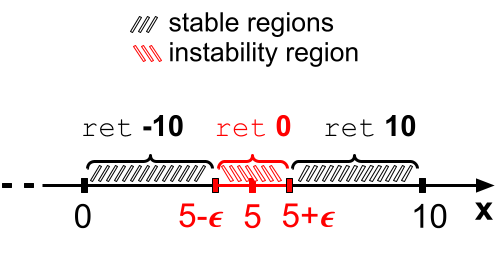
\includegraphics[width=0.48\textwidth]{pic/iffp.png}
	\end{tabular}
	\caption{The evaluation of a simple if-statement in case of real arithmetic (left) and the floating-point counterpart (right). You can see the instability region (in red), where $\epsilon$ is the roundoff error accumulated by the variable x.}
	\label{fig:ifreal}
\end{figure}
%
In Figure \ref{fig:ifreal}, we plot the instability region for the program. Clearly, when we compute in real arithmetic we do not have instabilities. On the other hand, in the floating-point program we can identify the \emph{instability region} as that part of the input domain from where instabilities might be triggered.
%
The width of the instability region is determined by the roundoff error $\epsilon$ accumulated by $x$. From Equation (\ref{standard}), we know the roundoff error is proportional to $x*e$, hence in the worst-case formulation, we have $\max(x*e) = x*\epsilon = x*(2^{-p})$, where p is the bit-width of the floating-point format. The error $\epsilon$ assumes maximal magnitude when $x=10$ and, in double precision floating-point arithmetic (64 bits), we get $\epsilon=1.11e^{-15}$.
%

We can use $\epsilon$ to make our program \emph{robust} to roundoff errors~\cite{guardstable}.
%
First, we identify the instability region, centered at 5 and with width $2\epsilon$, from where an instability might be triggered.
%
Any unstable execution stems from the instability region, but this is a conservative estimate, because also stable executions might land in the instability region.
%
\begin{figure}[b!]
	\begin{lstlisting}[frame=single, language=Python, escapeinside={(*}{*)}]
	x(*$\;\in\;$*)[0,10]
	if x>5+(*$\epsilon$*):
	  return 10
	elif x<(*$5-\epsilon$*):
	  return -10
	else: #we landed in the instability region
	  return 0
	\end{lstlisting}
	\caption{A \emph{robust} if-statement where the real execution and the floating-point counterpart always coincide.}
	\label{fig:ifrobust}
\end{figure}
%
Figure~\ref{fig:ifrobust} shows the robust program version, where the real-valued program and the floating-point counterpart always coincide. 
%
In other words, when the real program returns the value 10 also the floating-point counterpart returns 10. Similar argument holds for the return value -10.
%
Finally, the developer needs to consider the case where we land in the instability region, for example by using a special return value or a warning flag.
%
For the purpose of this example, we decide to return the value $0$ in the case where we land in the instability region. 

%On the other hand, the instability jump can be computed (statically) as $|10-(-10)|=20$. There are about 16 orders of magnitude between the roundoff error and the instability jump error.
%

Let us now slightly modify the range of the input variable x in our example. 
%
In particular, we set the range of x to the interval $[0, 10^{300}]$, and with a similar reasoning used so far, we compute the new width of the instability region and we get $\epsilon=7.43e^{283}$.
%
The width of the instability region is almost as wide as the max-representable value in double-precision, and of little use from an implementation perspective. 
%
Clearly, with this new value for $\epsilon$, the approach used so far to make the program \emph{robust} to roundoff errors is extremely conservative from an implementation perspective because almost all the computations, both the stable and the unstable ones, are going to land in the instability region.
%
Indeed, the robust program assumes \emph{any} computation landing in the instability region is unstable.
%
Moreover, the return value -10 becomes unreachable, meaning the robust program is never going to return -10.
%
%, which is also of little use from an implementation perspective.
%
This is because the condition $x<5-\epsilon$, leading to the return value -10, is always false when x is in $[0, 10^{300}]$ and $\epsilon=7.43e^{283}$.
%
Hence, by making the program robust to roundoff errors, we actually altered the logic of the original program.
%
A potential solution to tackle the conservative nature of static analysis without affecting the logic of the program would be to reason about instabilities using automated theorem provers.
%
Unfortunately, none of the existing engines can handle the mix of floating-point and real constraints.
%

%
In our contribution, we present FPRoCK, a prototype of a decision procedure for reasoning about the mix of real and floating-point constraints.
%
The innovative idea implemented in FPRoCK is the translation of a mixed formula with real and floating-point constraints into an equisatisfiable one over the reals.
%
The resulting formula, which contains only real constraints, is discharged to existing off-the-shelf SMT solvers for resolution.
%
We integrated FPRoCK on top of the static roundoff error analyzer PRECiSA~\cite{precisa} to reason about control-flow instabilities in floating-point programs.
%
FPRoCK works as a back-end solver for PRECiSA, and it is used to identify unfeasible (UNSAT) control-flow instabilities in conditional statements.
%
Thanks to FPRoCK, not only can we precisely reason about instabilities, but when an instability exists we also get a model triggering the instability.

\subsection{Application to Controller Synthesis}
\label{controllers}
%
Floating-point numerical algorithms are essential to many applications and it is often desirable to compute their results as accurately as possible.
%
Control-system designers using existing toolboxes, for example in MATLAB, use the well-known floating-point formats (single or double) as a proxy for real arithmetic. 
%
Indeed, at design time the main concerns are closed-loop performance and stability of the system.
%
%In the design of controller applications for embedded systems there is the need to take particular care for roundoff errors stemming from finite precision computations.
%
%Finite-precision numbers induce roundoff errors, and knowledge of the range of these roundoff errors is required to fulfill safety criteria of critical programs, as typically arising in modern embedded systems such as aircraft controllers.
%
On the other hand, from an implementation perspective, meaning when it is time to deploy the controller on the chip, other factors such as performance, hardware dimensions, and energy consumption become primary concerns~\cite{suardi}.
%
In the last decade there has been a massive usage of low precision floating-point formats, for example in artificial intelligence (AI), with the aim of conserving resources~\cite{fppower}.
%
Leveraging low precisions can lead to significant savings, and the impact of low-cost floating-point precisions on machine learning predictors is an active research area.
%
The natural question then would be whether we can \emph{implement} the \emph{ideal} controller (from MATLAB) using low-precision formats, while still guaranteeing the stability of the system.
%
In other words, in case we implement the controller using low-precision formats, would the controller still be able to govern the system for which it has been designed?
%
%where the user has to provide the floating-point format used to implem which aims to reduce memory usage
%in explicit MPC control, as it requires the user to provide a (uniform) "xed-precision up front. Instead, we
%let Daisy "nd the minimum uniform precision needed.
%

In our contribution, we embed the state-of-the-art for worst-case roundoff error analysis in the design process of linear time invariant (LTI) Model Predictive Controllers (MPC)~\cite{mpc}.
%
As opposed to the approach used in the state-of-the-art~\cite{suardi}, which requires the user to provide \emph{up front} the floating-point format to implement the MPC controller, in our work we rely on the fully automated \emph{precision-tuning} routine implemented in Daisy~\cite{darulova2018daisy}, to detect the most appropriate low-precision format to implement the controller.
%
The tool flow of our approach is briefly described in the following.

%
We measure the roundoff error stemming from the finite-precision implementation of the controller using static-analysis techniques, and then we include this error in the set of all the disturbances affecting the system.
%
In general, a robust MPC controller is designed to govern a system which is subject to various sources of external disturbances, for example, friction, wind resistance, and noisy sensors.
%
Hence, at design time, the designer of the controller estimates the total amount of disturbance $\Delta$ the controller has to handle.
%
Since $\Delta$ accounts for various sources of disturbance, it is also called the \textquotesingle\textquotesingle disturbance budget\textquotesingle\textquotesingle.
%
%Our idea consists in including the roundoff error stemming from the finite-precision implementation of the controller as an additional disturbance affecting the system.
%
In our framework, we use a fully automated precision tuning routine~\cite{fptuner} which reduces the bit-width format for the arithmetic and the memory foot-print of the controller until the saturation point is reached, where the roundoff error violates the budget delta.
%
This is going to be the most memory efficient low-precision controller which respects the disturbance budget $\Delta$, and thus the stability of the system is not affected.
%
%Furthermore, we use the so called mixed-precision tuning to further reduce the precision of the co, using the assumption that there might be only certain area that have to be computed precisely and not all of them.

%WORST-CASE ANALYSIS HAS NOT BEEN EMBEDDED IN REAL WORLD %APPLICATIONS (LIKE WHAT YOU DID IN EMSOFT).
%
%  
%  
%
%WE WANT TO HELP DEVELOPERS.
%
%LIMITATIONS OF WORST CASE ANALYSIS IN CASE OF DISTRIBUTION.
%
%
\subsection{Probabilistic Error Analysis}
\label{sec:prob}
%
In this section we describe the limitations of worst-case roundoff error analysis, and we introduce our framework to compute probabilistic roundoff error bounds.
%

Worst-case analysis can provide overly pessimistic error bounds in case we know \emph{a priori} the distribution of the input variables. 
%
%Furthermore, we must bound the input variables to prevent overflow and thus unbounded roundoff errors.
%
Figure~\ref{fig:prob} shows a simple program with a conditional statement we use to study the limitations of worst-case analysis.
%
\begin{figure}[b!]
	\begin{lstlisting}[frame=single, language=Python]
	if x>constant:
	  return 1/0 #ERROR
	else:
	  return 0 #OK
	\end{lstlisting}
	\caption{A simple if-statement we use to study the conservativeness of worst-case analysis. The \emph{then} branch leads to an error, while the \emph{else} branch returns correctly.}
	\label{fig:prob}
\end{figure}
%
We assume the variable $x\sim Normal(0,1)$ is distributed according to a standard normal with parameters $\mu = 0$ and $\sigma = 1$.
%
At line 1, we compare $x$ with a constant value, and in case the comparison evaluates to true the \emph{then} branch leads to an error (division by zero); otherwise, the \emph{else} branch returns correctly.
%
\emph{Regardless} of the value of the constant used for the comparison, \emph{any} rigorous (i.e. sound) worst-case range analysis is going to signal a potential division-by-zero error at line 2.
%
In other words, the worst-case analysis is going to terminate as soon as a potential division by zero is detected.
%
This is because, in case the error at line 2 is triggered at runtime, the program would crash, hence it would not make sense to reason about ranges or roundoff errors.
%
A developer using such worst-case tools does not get any information about \emph{how rare} the condition leading to such a crash might be.
%
This is due to the nature of worst-case analysis, where there is no distinction between extremely rare or average computations.
%

To tackle these limitations we need a \emph{probabilistic} error analysis.
%
The only existing work in the state-of-the-art, apart from the contribution described in this dissertation, is the rigorous probabilistic error analysis called PrAn~\cite{probdaisy}.
%
Unfortunately, PrAn heavily relies on the underlying worst-case error analysis implemented in Daisy~\cite{darulova2018daisy}, thus PrAn inherits some of the limitations of worst-case analysis, in particular, the conservativeness of the error bounds.
%
The immediate consequence is that the probabilistic errors from PrAn are always in the same order of magnitude of the worst-case errors from Daisy.
%

In our framework, we use probabilistic range analysis to compute average roundoff errors where, as opposed to the worst-case approach, the roundoff error is estimated with respect to the computation landing in a given confidence interval of interest (e.g., 85\%, 99\%, 99.9999\%).
%
Note, in the worst-case approach there is an implicit 100\% confidence interval, thus worst-case analysis and 100\% confidence interval are synonymous.
%
In our probabilistic framework, we know the standard normal distribution concentrates more than 99\% of probability mass in the interval $[-3, 3]$, and less than 0.5\% of mass spreads in the interval $[3, \infty]$.
%
If we go back to our example, if at line 1 we set the constant to 1000, a developer using our combined analysis might not be interested in the very rare outliers leading to the error at line 2.
%
Thus, we can run our probabilistic analysis with a \emph{confidence interval} set, for example, to 99\%, and not only will the program terminate correctly (return 0), but our probabilistic error bound is $\epsilon = x*(2^{-p}) = 3*(2^{-p})$ which in double precision leads to $\epsilon = 3.33e^{-16}$.
%
Note how when we run worst-case analysis without bounding the variable $x$, we would get an infinite error bound, which is of little use from an implementation perspective. 
%
In general, by studying the \emph{average} execution of a computer program we can prune away very rare corner cases and provide meaningful directions to the developer.
%
\newpage
\bibliographystyle{acm}
\bibliography{\jobname}

%When we trade the accuracy of a computation for efficiency, what can we say about property of our system like stability or soundness. In alternative, in case we cannot guarantee soundness anymore, can we measure exactly how much unsoundness our application has to be able to tolerate.
%
%This is critical when we want to bound roundoff errors for programs rather than for arithmetic expressions.
%
%We use 
%

%
%Efficiently collecting data and systematically analyzing them is essential to gaining insight into the behavior of complex programs and help developers fix the flaws of the program. Also, given the rich set of concurrency primitives in modern languages, one needs to articulate nuanced concurrency coverage metrics and demonstrate their attainment.
%
%And this is my thesis statement: exact reasoning about roundoff error is hard. We can use exact reasoning for handling conditionals (like we show with FPRock). Overapproximation works for real world problem, like EMSOFT, but it is worst-case. We show how a probabilistic analysis can tackle the limitations of worst-case analyisis in real world applications.